% (c) 2015 Daniele Zambelli daniele.zambelli@gmail.com

\input{\folder luoghigeometrici_grafici.tex}

\chapter{Complementi sulle coniche}
\label{sec:coniche}

\section{Le posizioni di una retta rispetto ad una conica}
\label{sec:coniche_e_retta}

Studiamo ora le posizioni reciproche tra una retta ed una conica, entrambe 
giacenti sullo stesso piano. Consideriamo ad esempio il caso di una retta 
ed un'ellisse sullo stesso piano; le situazioni che si possono verificare 
sono tre:
\begin{itemize} [noitemsep]
  \item la retta passa esternamente alla conica e non ha alcun 
punto in comune con la conica (si definisce \emph{esterna});
  \item la retta tocca la conica in un solo punto
 (si definisce \emph{tangente});
  \item la retta interseca la conica in due punti  (si definisce \emph{secante}).
  \end{itemize}
  
\begin{figure}[htbp]
  \centering
  %    \begin{inaccessibleblock}[Cono a due falde tagliato da un piano
  %      che forma un'ellisse.]
  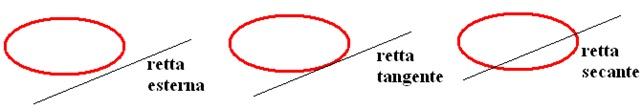
\includegraphics[width=\textwidth]{img/rettaconica.jpg}
  \caption{Posizioni reciproche tra una retta ed un'ellisse.}%
  %\label{fig:ellissedalcono}
  %    \end{inaccessibleblock}
\end{figure}
Geometricamente, per stabilire la posizione di una retta rispetto ad una 
conica, disegniamo i due oggetti sul piano cartesiano e verifichiamo quanti 
punti hanno in comune. Algebricamente, per stabilire la posizione di una 
retta rispetto a una conica andiamo a considerare il sistema delle due 
equazioni: quella della conica (ad esempio un'ellisse) e quella della 
retta:
\[\begin{cases}  \dfrac{x^{2}}{a^{2}}+\dfrac{y^{2}}{b^{2}}=1   \\ y=mx+q  
\end{cases}\]
Il sistema da' luogo ad un'equazione di secondo grado, nella quale il 
segno di \(\Delta\) determina la posizione reciproca fra i due oggetti:

\begin{itemize} [noitemsep]
  \item se \(\Delta<0\), l'equazione di secondo grado non ha soluzioni 
reali: retta e conica non hanno punti in comune, non si intersecano;
  \item se \(\Delta=0\), l'equazione di secondo grado ha due soluzioni coincidenti: conica e retta hanno un solo 
punto in comune: la retta è tangente alla conica;
  \item se \(\Delta>0\), l'equazione di secondo grado ha due soluzioni:
  i punti in comune tra retta e conica sono due: la retta è 
secante alla conica.
\end{itemize}

In generale per determinare le intersezioni tra retta e conica, 
determinandone così la posizione relativa, 
dobbiamo risolvere un sistema a due equazioni: quella della conica e quella 
della retta. 

\begin{esempio} Data la parabola \( y = x^2-3x-4\) e la retta \(y=x+2\), stabilire la posizione della retta 
rispetto all'ellisse.
\\[7pt]
Innanzitutto dobbiamo costruire un sistema con le due equazioni date, e iniziare a risolvere:
\[\begin{cases} y =x^2-3x-4 \\ y=x+2\end{cases} \quad \Rightarrow \quad \begin{cases} x+2 =x^2-3x-4 \\ y=x+2\end{cases}\]
Prendiamo solamente la prima equazione, e calcoliamone il valore di \(\Delta\):
\[x+2 =x^2-3x-4 \quad \Rightarrow \quad x^2-4x-6=0 \quad \Rightarrow \quad \Delta = 16+24=40>0\]
Poiché \(\Delta>0\) le due curve sono secanti.
\end{esempio}

% Per fare una ulteriore applicazione studiamo le intersezioni tra una 
% parabola e una retta.
% Data la parabola di equazione P: y=a\( x^{2}+bx+c\) e la retta generica \(r\): 
% y=mx+q le loro intersezioni sono determinate dal sistema:
% \[\begin{cases}  y=a x^{2} +bx+c   \\ y=mx+q  
% \end{cases}\]
% dal quale otteniamo l'equazione:
% \(ax^{2} +(b-m)x+c-q=0\)
% equazione di secondo grado in x, le cui soluzioni sono le ascisse dei punti 
% di intersezione, a seconda del segno del \( \Delta \) dell'equazione ci 
% saranno due soluzioni nel caso di retta secante, una nel caso di retta 
% tangente e nessuna nel caso di retta esterna, come mostrato nela seguente 
% figura:
% \begin{figure}[htbp]
%   \centering
%   %    \begin{inaccessibleblock}[Cono a due falde tagliato da un piano
%   %      che forma un'ellisse.]
%   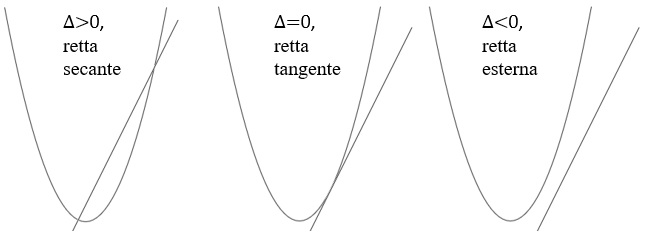
\includegraphics[scale=0.6]{img/rettaconica3.jpg}
%   \caption{Posizioni reciproche tra una retta ed una parabola.}%
%   %\label{fig:ellissedalcono}
%   %    \end{inaccessibleblock}
% \end{figure}

\begin{esempio} Data l'ellisse \( \dfrac{x^{2}}{16}+  
\dfrac{y^{2}}{4} =1\) e la retta \(y=x+4\), stabilire la posizione della retta 
rispetto all'ellisse e calcolare le coordinate degli eventuali punti di intersezione.\\[7pt] 
Secondo quanto visto il sistema da risolvere è:
\(\begin{cases}  \dfrac{x^{2}}{16}+\dfrac{y^{2}}{4}=1   \\ y=x+4  
\end{cases}\) \\[4pt]
sostituendo otteniamo l'equazione: \( 
\dfrac{x^{2}}{16}+\dfrac{x^{2}+8x+16}{4}=1 \quad \Rightarrow \quad 5 
x^{2} +32x+48=0\)\\[7pt]
Calcoliamo dunque il valore di \(\Delta\): \(\quad \Delta =1024-960=64>0\). \\[7pt]
\begin{minipage}{.65\textwidth}
\noindent La retta è dunque secante. Calcoliamo ora i due punti di 
intersezione. Risolvendo l'equazione precedente otteniamo le ascisse dei punti di 
intersezione: \( x_{1} =- \dfrac{12}{5} \) e \( x_{2} =-4\). Sostituendo tali 
ascisse nell'equazione della retta otteniamo le corrispondenti ordinate \( 
y_{1} =\dfrac{8}{5}\) e \( y_{2} =0\). I punti cercati sono quindi: \( P_{1}  
\left(-\dfrac{12}{5};~ \dfrac{8}{5}\right) \) e \( P_{2} =(-4;~0)\).
\end{minipage}
\hspace{0.5cm}
\begin{minipage}{.35\textwidth}
  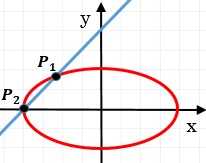
\includegraphics[width=\textwidth]{img/esempioposizione1.jpg}
  %    \caption{Generazione di un cono a due falde}% 
\end{minipage}
\end{esempio}
 
\section{Rette tangenti ad una conica}
\label{sec:coniche_tangenti}

Analizziamo, nello specifico, il caso di tangenza. In generale, per un 
punto esterno ad una conica, possono esser condotte due tangenti mentre, per 
un punto appartenente alla conica, può essere condotta una sola tangente;  
da un punto interno alla conica, cioè dalla sua parte convessa, non si 
possono tracciare tangenti, come illustrato in Figura \ref{fig:ellissedalcono} nel caso della 
parabola. 

\begin{figure}[t]
  \centering
  %    \begin{inaccessibleblock}[Cono a due falde tagliato da un piano
  %      che forma un'ellisse.]
  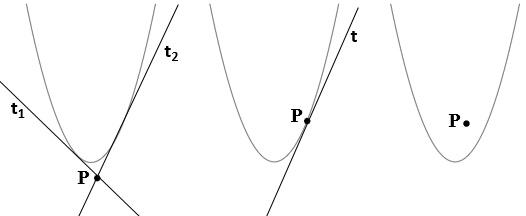
\includegraphics[scale=0.8]{img/tangenti2.jpg}
  \caption{Rette tangenti alla parabola.}%
  \label{fig:ellissedalcono}
  %    \end{inaccessibleblock}
\end{figure}

Quanto appena visto per la parabola vale anche per le altre coniche.
Vogliamo ora determinare le rette tangenti ad una conica passanti per un 
punto dato. I casi possibili, come abbiamo appena visto, sono due: se il 
punto è esterno alla conica, in generale, si trovano due rette tangenti, se 
il punto appartiene alla conica, una sola tangente.

\subsection{Tangenti per un punto esterno ad una conica}

Per un punto esterno ad una conica passano due rette tangenti alla conica 
stessa. Per determinare le equazioni di queste tangenti, conoscendo la 
conica e le coordinate del punto esterno, in generale, si procede con il 
metodo del \( \Delta =0\). Andiamo ad illustrare per punti tale metodo:

\begin{itemize} [noitemsep]
  \item si scrive l'equazione del fascio proprio di rette centrato 
nel punto dato, avente \(m\) come parametro non noto: \(y- y_{0} =m\left(x-x_{0}\right)\);
  \item si mette a sistema tale equazione con quella della conica 
data;
  \item si risolve il sistema per una variabile, \(x\) o \(y\), trovando un'equazione
  di secondo grado ad un parametro (\(m\)) e si determina il \( \Delta \) 
di tale equazione;
  \item ponendo \( \Delta =0\) si determinano i valori del parametro \(m\) 
che costituiscono i coefficienti angolari delle rette tangenti cercate. Si calcolano quindi
le equazioni di tali rette sostituendo i valori di \(m\) appena trovati nell'equazione del fascio di 
rette iniziale.
\end{itemize}

  Poniamo attenzione a quest'ultimo punto. Se l'equazione 
del \( \Delta =0\) è di secondo grado in \(m\), i due valori di \(m\) rappresentano i 
coefficienti angolari delle due rette. Se invece l'equazione è di 
primo grado la sua soluzione rappresenterà il coefficiente di una sola retta 
tangente mentre l'altra tangente sarà fornita dalla retta verticale \(x= 
x_{0} \). Nella formula del fascio di rette infatti non è mai compresa la 
retta verticale passante per il centro del fascio. Tale retta, per 
completare il fascio, andrebbe aggiunta alla formula del fascio:
\[\quadra{\;y-y_{0} =m(x- x_{0} )\;}\; \cup\; \quadra{\;x= x_{0}\;} \]
  

\begin{esempio} Determinare le equazioni delle tangenti 
all'ellisse \( x^{2} + \dfrac{y^{2}}{3} \)=1 condotte da \(P(2;~0)\).
\\[7pt]
Procediamo come appena indicato. Il fascio di rette di centro 
P è dato da:
\[y-0=m(x-2)\quad \cup  \quad x=2\] 
Tralasciando per ora la retta verticale,
costruiamo il sistema con le due equazioni (fascio e conica):
\[\begin{cases}  x^{2}+\dfrac{y^{2}}{3}=1   \\ y=mx-2m  
\end{cases} \sRarrow  
\begin{cases}  3x^{2}+y^{2}=3   \\ y=mx-2m  
\end{cases} \sRarrow  
\begin{cases}  3x^{2}+m^{2}x^{2}+4m^{2}-4m^{2}x-3=0   \\ y=mx-2m  
\end{cases}\]
Riscriviamo l'equazione di secondo grado ottenuta, trovandone il \(\Delta\) 
con la formula ridotta (\(\frac{\Delta}{4}\)):
\[\tonda{3+ m^{2} } x^{2} -4 m^{2} x+\tonda{4 m^{2} -3}=0\] 
\[\Delta =4 m^{4} -(3+ m^{2} )(4m^{2}-3)=
4 m^{4} -12 m^{2} +9-4 m^{4} +3 m^{2} =-9 m^{2} +9\]. 
Ponendolo uguale a zero, e risolvendo 
l'equazione successiva, otteniamo: \(m_{1} = 1\) e \(m_{2} = -1\).
Sostituiamo i valori di \(m\) appena trovati nell'equazione del fascio per trovare le 
due corrispondenti rette tangenti: \(y=x-2\) e \(y=-x+2\).
\end{esempio}

\begin{esempio} Determinare le equazioni delle tangenti 
all'ellisse \(x^{2} + \dfrac{y^{2}}{3} =1\) condotte da 
\(P\punto{1}{2}\).\\[7pt]
L'equazione del fascio di rette di centro \(P\) è:  \(\quad y-2=m(x-1)\quad \cup \quad x=1\)\\[3pt]
Tralasciando ancora una volta la retta verticale, il sistema che si ottiene, mettendo insieme conica e fascio, è:
\[\begin{cases}  x^{2}+\dfrac{y^{2}}{3}=1   \\ y=mx-m+2  
\end{cases} \sRarrow  
\begin{cases}  3x^{2}+y^{2}=3   \\ y=mx-m+2  
\end{cases} \sRarrow 
\begin{cases}  3x^{2}+\tonda{mx-m+2}^2=3   \\ y=mx-m+2  
\end{cases}\]
l'equazione di secondo grado, con i termini già raccolti, risulta: 
\[\left(3+ m^{2} \right) x^{2} +2\left(2m-m^{2} \right)x+ \tonda{m^{2} -4m+1}=0\]
Calcolandone il \(\Delta\) della formula ridotta si ha dunque:
\[\begin{split}
\Delta & = \tonda{2m-m^{2}}^2 -\tonda{3+ m^{2}}\tonda{m^{2}-4m+1} \\
 & =4 m^{2} + m^{4} -4 m^{3} -3 m^{2} +12m-3- m^{4} +4 m^{3} - m^{2} \\&=12m-3
\end{split}\]
Ponendo ora \(\Delta =0\), otteniamo \(m=\dfrac{1}{4}\). La corrispondente retta tangente è:
\[y-2=\dfrac{1}{4}(x-1) \longrightarrow  4y-x-7=0\]
Il punto \(P\) è esterno alla conica, quindi non può esserci solamente una retta tangente.\\
Di conseguenza la seconda retta tangente è la retta verticale inizialmente omessa: \(x=1\).
\end{esempio}

\subsection{Tangente per un punto appartenente alla conica}

Se il punto, per il quale si vogliono cercare le tangenti ad una conica, 
appartiene alla conica stessa, necessariamente la soluzione sarà univoca. 
Per trovare tale retta si può ricorrere ancora al metodo precedente del \( \Delta =0\) ma si 
preferisce, in questo caso, usare il meno complesso \emph{metodo dello 
sdoppiamento}. Tale metodo evita di impostare e risolvere il sistema a due 
equazioni di secondo grado e con una semplice sostituzione permetter di ricavare 
immediatamente la retta tangente cercata.
Andiamo ad illustrare per punti tale metodo, utilizzando come esempio una circonferenza,
ma sottolineando subito che tale metodo può essere applicato ad una qualunque conica:

\begin{itemize} [noitemsep]
  \item  Dato il punto \(P( x_{0};~ y_{0} )\) appartenente alla 
circonferenza e scritta l'equazione canonica della circonferenza \( x^{2} + 
y^{2} +ax+by+c=0\) si procede con le seguenti sostituzioni:
\[ x^{2} \longrightarrow x x_{0}  \quad ;\quad y^{2} \longrightarrow y y_{0}\quad ;\quad
x= \dfrac{x+x_{0}}{2} \quad ;\quad y= \dfrac{y+y_{0}}{2}\]

  \item Si ottiene così la seguente equazione che rappresenta la retta 
tangente cercata:
 \[x x_{0} +y y_{0}+a\; \dfrac{x+x_{0}}{2}  +b\; \dfrac{y+y_{0}}{2} +c=0\]
\end{itemize}

\begin{minipage}{.40\textwidth}
\begin{esempio} Determinare l' equazione della tangente 
all'ellisse 
\[\dfrac{x^{2}}{100}+\dfrac{y^{2}}{25} =1\]
assante per il suo punto \(P\) di coordinate \(P\left(6;~4\right)\).

\noindent
Procediamo come appena indicato, mediante metodo di sdoppiamento. 
Sostituendo:
\end{esempio}
\end{minipage}
\hfill
\begin{minipage}{.58\textwidth}
\begin{center} \luoghitangente \end{center}
\end{minipage}
\[\dfrac{xx_{0}}{100} + \dfrac{yy_{0}}{25} = 1 \quad \rightarrow \quad
\dfrac{6x}{100} + \dfrac{4y}{25} =1 \quad \rightarrow \quad 
\dfrac{3x}{50}+\dfrac{8y}{50}=1\quad \rightarrow \quad 3x+8y-50=0\]
Che esplicitando y diventa:
\[y=-\frac{3}{8}x+\frac{25}{4} \quad \rightarrow \quad 
y=-\frac{3}{8}x+6+\frac{1}{4}\]

\section{Funzioni deducibili dalle equazioni delle coniche}
\label{sec:coniche_curve_deducibili}

La conoscenza delle equazioni e delle proprietà delle coniche consente di 
rappresentare graficamente alcune tipologie di funzioni irrazionali.\\
\begin{esempio} Tracciamo il grafico della funzione 
\(y=\sqrt{4-9x^{2}}\).\\[7pt] Innanzitutto la funzione è definita solo se il 
radicando è non negativo, ovvero \(4-9x^{2}\geq0\). Il secondo membro 
dell'equazione di conseguenza risulta essere non negativo. Per mantenere l'uguaglianza 
anche il primo membro deve essere non negativo, quindi \( y\geq 0 \). 
A questo punto, con le condizioni poste, possiamo elevare al quadrato entrambi i membri dell'equazione
per eliminare la radice, ottenendo \( y^{2}=4-9x^{2} \) che non è altro che 
l'equazione di un'ellisse: \( 9x^{2}+y^{2}=4 \).
\\[5pt]
Quanto appena visto equivale all'impostazione del sistema:\\[7pt]
% \begin{figure} [h]
\noindent \begin{minipage}{.7\textwidth}
\[\begin{cases}  4-9x^{2}\geq 0   \\ y\geq0  \\y^{2}=4-9x^{2} 
\end{cases} \sRarrow
\begin{cases}   -\dfrac{2}{3}\leq x\leq \dfrac{2}{3}   \\ y\geq0  \\ 
9x^{2}+y^{2}=4 \end{cases}\] 
La soluzione grafica di questo sistema è un'ellisse che ha 
dei limiti sia in ascissa che in ordinata. Per tener conto di \( y\geq0 \) 
dobbiamo prendere solo la parte dell'ellisse con ordinata positiva o nulla, 
cioè la parte di ellisse contenuta nel primo e secondo quadrante; i limiti sulle ascisse
sono invece già verificati per ogni punto della stessa.
  \end{minipage}
  \hspace{.7cm}
  \begin{minipage}{.3\textwidth}
    %    \begin{inaccessibleblock}[Cono a due falde tagliato da un piano
    %      che forma un'ellisse.]
    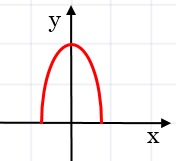
\includegraphics[width=.85\textwidth]{img/curva1.jpg}
%     \caption{Grafico dell'equazione \( y=\sqrt{4-9x^{2}} \).}
    %\label{fig:ellissedalcono}
    %    \end{inaccessibleblock} 
  \end{minipage}
% \end{figure}

\end{esempio}

\begin{esempio} Disegnare il grafico di \(y=2-\sqrt{6x-x^{2}} \).\\[7pt]Come primo passo riscriviamo la 
funzione come \(y-2=-\sqrt{6x-x^{2}}  \), poi cerchiamo di impostare un 
sistema simile al precedente che rispetti le condizioni di esistenza del 
radicale e le sue conseguenze:
\[\begin{cases}  6x-x^{2}\geq0   \\ y-2\leq0  \\y^{2}-4y+4=6x-x^{2} 
\end{cases} \sRarrow
\begin{cases}   0\leq x\leq6   \\ y\leq2  \\ x^{2}+y^{2}-6x-4y+4=0 
\end{cases}\]

% \begin{figure} [h]
\noindent \begin{minipage}{.7\textwidth}
La prima disequazione rappresenta di nuovo le condizioni del 
radicale, la seconda disequazione ci ricorda che il primo membro, \(y-2\), deve 
avere lo stesso segno del secondo (che essendo una radice con segno 
negativo davanti, non può essere positivo), infine l'equazione rappresenta 
una circonferenza di centro \(\punto{3}{2}\) e raggio \(3\). Il grafico cercato è dunque quello di una 
circonferenza, limitata nelle ordinate a 
\(y\leq2\).
  \end{minipage}
  \hfill
  \begin{minipage}{.25\textwidth}
    %    \begin{inaccessibleblock}[Cono a due falde tagliato da un piano
    %      che forma un'ellisse.]
    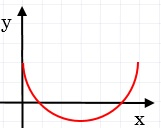
\includegraphics[width=\textwidth]{img/curva2.jpg}
%     \caption{Grafico dell'equazione \( y=2-\sqrt{6x-x^{2}} \).}
    %\label{fig:ellissedalcono}
    %    \end{inaccessibleblock} 
  \end{minipage}
% \end{figure}

\end{esempio}

% \begin{figure} [h]
\begin{esempio} Disegnare il grafico di \( y=\sqrt{4-x} \).\\[7pt]
\begin{minipage}{.65\textwidth}
\noindent  Costruiamo subito il sistema 
corrispondente:
\[\begin{cases}  4-x\geq0   \\ y\geq0  \\y^{2}=4-x 
\end{cases} \sRarrow
\begin{cases}   x\leq4   \\ y\geq0  \\ x=-y^{2}+4 
\end{cases}\]
otteniamo una parabola con l'asse parallelo all'asse \(Y\), di cui 
prendiamo in considerazione solo la parte con \(y\) non negativa.
  \end{minipage} \hspace{.7cm}
  \begin{minipage}{.25\textwidth}
  %    \begin{inaccessibleblock}[Cono a due falde tagliato da un piano
  %      che forma un'ellisse.]
  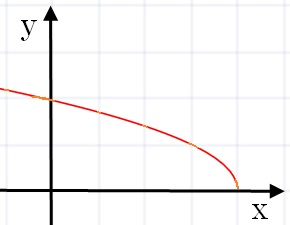
\includegraphics[width=\textwidth]{img/curva3.jpg}
%   \caption{Grafico dell'equazione \( y=\sqrt{4-x} \).}
  %\label{fig:ellissedalcono}
  %    \end{inaccessibleblock} 
\end{minipage}
  \end{esempio}
% \end{figure}


